\documentclass[runningheads]{llncs}

% ---------------------------------------------------------------
% Include basic ECCV package
 
% TODO REVIEW: Insert your submission number below by replacing '*****'
% TODO FINAL: Comment out the following line for the camera-ready version
\usepackage[review,year=2026,ID=*****]{eccv}
% TODO FINAL: Un-comment the following line for the camera-ready version
%\usepackage{eccv}

% OPTIONAL: Un-comment the following line for a version which is easier to read
% on small portrait-orientation screens (e.g., mobile phones, or beside other windows)
%\usepackage[mobile]{eccv}


% ---------------------------------------------------------------
% Other packages

% Commonly used abbreviations (\eg, \ie, \etc, \cf, \etal, etc.)
\usepackage{eccvabbrv}

% Include other packages here, before hyperref.
\usepackage{graphicx}
\usepackage{booktabs}
\usepackage{amsmath}
\usepackage{amssymb}

% The "axessiblity" package can be found at: https://ctan.org/pkg/axessibility?lang=en
\usepackage[accsupp]{axessibility}  % Improves PDF readability for those with disabilities.


% ---------------------------------------------------------------
% Hyperref package

% It is strongly recommended to use hyperref, especially for the review version.
% Please disable hyperref *only* if you encounter grave issues.
% hyperref with option pagebackref eases the reviewers' job, but should be disabled for the final version.
%
% If you comment hyperref and then uncomment it, you should delete
% main.aux before re-running LaTeX.
% (Or just hit 'q' on the first LaTeX run, let it finish, and you
%  should be clear).

% TODO FINAL: Comment out the following line for the camera-ready version
%\usepackage[pagebackref,breaklinks,colorlinks,citecolor=eccvblue]{hyperref}
% TODO FINAL: Un-comment the following line for the camera-ready version
\usepackage{hyperref}

% Support for ORCID icon
\usepackage{orcidlink}


\begin{document}

% ---------------------------------------------------------------
% TODO REVIEW: Replace with your title
\title{Author Guidelines for ECCV Submission} 

% TODO REVIEW: If the paper title is too long for the running head, you can set
% an abbreviated paper title here. If not, comment out.
\titlerunning{Abbreviated paper title}

% TODO FINAL: Replace with your author list. 
% Include the authors' OCRID for the camera-ready version, if at all possible.
\author{First Author\inst{1}\orcidlink{0000-1111-2222-3333} \and
Second Author\inst{2,3}\orcidlink{1111-2222-3333-4444} \and
Third Author\inst{3}\orcidlink{2222--3333-4444-5555}}

% TODO FINAL: Replace with an abbreviated list of authors.
\authorrunning{F.~Author et al.}
% First names are abbreviated in the running head.
% If there are more than two authors, 'et al.' is used.

% TODO FINAL: Replace with your institution list.
\institute{Princeton University, Princeton NJ 08544, USA \and
Springer Heidelberg, Tiergartenstr.~17, 69121 Heidelberg, Germany
\email{lncs@springer.com}\\
\url{http://www.springer.com/gp/computer-science/lncs} \and
ABC Institute, Rupert-Karls-University Heidelberg, Heidelberg, Germany\\
\email{\{abc,lncs\}@uni-heidelberg.de}}

\maketitle


\begin{abstract}
  The abstract should concisely summarize the contents of the paper. 
  While there is no fixed length restriction for the abstract, it is recommended to limit your abstract to approximately 150 words.
  Please include keywords as in the example below. 
  This is required for papers in LNCS proceedings.
  \keywords{First keyword \and Second keyword \and Third keyword}
\end{abstract}


\section{Introduction}
\label{sec:intro}

Multi-camera 3D perception is a core requirement for intelligent transportation
systems, robotic warehouses, and large indoor smart spaces. In these environments,
a single camera rarely observes the full scene, and objects often move across
overlapping and non-overlapping fields of view~\cite{tang2019cityflow,chavdarova2018wildtrack}.
A useful perception system must therefore detect objects in individual images,
lift them into a shared world coordinate system, and maintain consistent identities
over time~\cite{hou2020mvdet,hou2021mvdetr,wang2024bevsushi}. This requirement
makes the task more difficult than standard 2D detection, because success depends
not only on recognizing objects, but also on accurate 3D localization and reliable
cross-camera association.

AI City Challenge 2026 Track 1 captures this difficulty through a sim-to-real
multi-camera 3D tracking setting~\cite{aicity2026track1}. The training and
validation data are collected from synthetic warehouse environments, while the
test data are real-world videos from calibrated multi-camera scenes. This setting
creates a direct domain gap between the visual appearance seen during training and
the visual appearance encountered during evaluation~\cite{tobin2017domainrandomization,hoffman2018cycada}.
At the same time, the output format requires global 3D bounding boxes with object
identities, so errors in 2D detection, camera projection, 3D lifting, and temporal
association all affect the final 3D Higher Order Tracking Accuracy (HOTA) score,
which jointly measures detection, association, and localization
quality~\cite{luiten2021hota}. As a result, the challenge is not only to build a
strong detector, but to build a complete perception pipeline that remains reliable
when synthetic supervision is transferred to real camera networks.

Existing multi-camera 3D tracking methods often address this problem by combining
image detections, camera calibration, depth information, bird's-eye-view (BEV)
aggregation, and tracklet association~\cite{wang2024bevsushi,wang2025mcblt,phan2025vgcrtrack,
tran2025depthtrack,vuminh2025online3d,lee2025pointcloud}. These components are
effective when their assumptions are well matched to the data. However, in a
sim-to-real setting, each component can introduce a different type of error. A
detector trained on synthetic data may miss rare object classes or produce poorly
calibrated confidence scores on real images~\cite{guo2017calibration,ovadia2019uncertainty,
lee2025pointcloud}. A depth-based lifting module may be sensitive to the depth
source, camera alignment, or representation mismatch between synthetic and real
scenes~\cite{phan2025vgcrtrack,tran2025depthtrack,vuminh2025online3d}. A tracker
may also create fragmented identities when uncertain detections are discarded or
treated in the same way as stable multi-view observations~\cite{zhang2022bytetrack,
cetintas2023sushi}. These failure modes suggest that the central problem is not
only how to obtain more detections, but how to preserve and use reliability
information throughout the full 3D tracking pipeline.

Our work is motivated by this observation. In calibrated multi-camera scenes,
object candidates have different levels of geometric support. Some candidates are
detected with high confidence, agree across multiple cameras, project consistently
into the world frame, and remain stable across nearby frames~\cite{hou2020mvdet,
hou2021mvdetr,wang2024bevsushi}. Other candidates are visible from only one camera,
have low confidence, appear near occlusion boundaries, or produce unstable 3D
locations after lifting. Treating these cases equally can increase false positives,
fragment identities, and reduce localization quality~\cite{zhang2022bytetrack,
cetintas2023sushi,wang2025mcblt}. A stronger pipeline should therefore propagate
reliability from 2D detection to 3D fusion, from 3D fusion to temporal assignment,
and from temporal assignment to track birth and track continuation.

Based on this view, we propose STAR-3D, a reliability-guided RGB-only framework
for multi-camera 3D tracking under sim-to-real shift. The method first applies
high-resolution object detection using complementary detector families, where a
recall-oriented detector and a precision-oriented detector are fused to improve
coverage while suppressing unstable boxes~\cite{solovyev2021wbf,peng2025dfine}.
The fused 2D detections are then lifted into the global coordinate system using the
provided camera calibration and class-specific 3D size priors. During multi-view
fusion, each 3D candidate is assigned reliability factors based on detector
confidence, camera support, spatial compactness, and consistency with plausible
object geometry. These reliability factors are not discarded after fusion.
Instead, they are carried into a class-conditioned tracker that adapts association
gates, track memory, and birth decisions according to object category and
observation stability.

This work makes the following contributions:
\begin{enumerate}
    \item We formulate sim-to-real multi-camera 3D tracking as a reliability
    propagation problem, where uncertainty from detection, projection, fusion,
    and association must be preserved rather than discarded.
    \item We propose STAR-3D, a calibrated RGB-only tracking framework that
    combines high-resolution heterogeneous detector fusion, reliability-guided
    multi-view 3D lifting, and class-conditioned causal association.
    \item We introduce a conservative bird's-eye-view tracklet graph refinement
    module that reduces identity fragmentation by linking only geometrically and
    temporally consistent tracklets.
    \item We provide an empirical analysis of depth-based and RGB-only strategies
    for AI City Challenge 2026 Track 1, showing that naive depth injection can hurt
    3D HOTA when depth, calibration, and detector confidence are not jointly
    calibrated.
\end{enumerate}

\section{Related Work}
\label{sec:related_work}

\subsection{Calibrated Multi-Camera 3D Perception}
\label{sec:related_multicamera}

Calibrated multi-camera perception builds on the classical observation that
multiple images of a shared scene can be related through camera geometry. The
foundations of this view are well established in projective geometry and camera
calibration, where intrinsic and extrinsic parameters make it possible to map
measurements between image coordinates and a common world frame~\cite{hartley2004multiple,
zhang2000calibration}. This geometric structure is especially important in
surveillance, traffic, and warehouse settings, because the same object may be
partially visible in one camera, fully visible in another camera, and absent in a
third. Early multi-camera benchmarks therefore emphasized synchronized video,
camera calibration, and identity consistency as central requirements for robust
perception~\cite{ristani2016dukemtmc,chavdarova2018wildtrack,tang2019cityflow}.
These datasets made clear that multi-camera perception is not simply a larger
version of single-view detection. It requires a representation in which evidence
from different cameras can be compared, fused, and tracked in a physically
meaningful coordinate system.

Early deep multi-view detection methods approached this problem by projecting
image evidence onto a ground plane and resolving occlusion through joint reasoning.
Deep occlusion reasoning showed that multi-camera information can reduce
ambiguities that remain difficult in crowded single-view images~\cite{baque2017deepocclusion}.
MVDet then made this idea more direct by learning feature perspective
transformations from each camera into a shared bird's-eye-view grid~\cite{hou2020mvdet}.
Because this projection created an explicit scene-level representation, the
network could aggregate support from multiple views before predicting object
locations. MVDeTr extended the same line of work with transformer-based
aggregation and view-coherent augmentation, allowing the model to adapt its
attention to camera-dependent projection distortions~\cite{hou2021mvdetr}.
Together, these works established the main design pattern behind calibrated
multi-camera detection: project each camera into a shared geometric space, fuse
multi-view evidence there, and predict objects in that common space.

The same design pattern also became central in autonomous-driving 3D perception,
where multi-camera rigs observe the surrounding scene from complementary
directions. Lift-Splat-Shoot introduced a differentiable image-to-BEV pipeline
that lifts image features into 3D frustums and splats them into a common BEV
representation~\cite{philion2020lift}. DETR3D took a query-based alternative by
using sparse 3D object queries to sample image features through calibrated
camera projections~\cite{wang2022detr3d}. BEVFormer further showed that
spatiotemporal transformers can learn BEV features from multi-camera images,
while PETR encoded 3D positional information into image features to support
end-to-end 3D object detection~\cite{li2022bevformer,liu2022petr}. BEVDepth
then highlighted the importance of reliable depth estimation for camera-based
BEV detection, and BEVFusion showed that a shared BEV representation can unify
camera and LiDAR information for multiple 3D perception tasks~\cite{li2023bevdepth,
liu2023bevfusion}. These methods demonstrate the strength of learned BEV
representations, but they are often developed for vehicle-mounted sensor rigs
with dense benchmarks, repeated camera layouts, and training distributions that
are closer to the evaluation domain than the sim-to-real warehouse setting.

Point-cloud 3D detection and tracking provide another important reference point
for multi-camera 3D perception. Methods such as PointPillars and CenterPoint
show that accurate 3D boxes can be obtained when metric 3D measurements are
available directly from LiDAR or point clouds~\cite{lang2019pointpillars,
yin2021centerpoint}. Tracking systems such as AB3DMOT further show that simple
motion models and Hungarian assignment can be highly effective once 3D detections
are already reliable~\cite{weng2020ab3dmot}. This line of work clarifies why 3D
localization quality is so important for HOTA-style evaluation: association can
become much easier when object centers, dimensions, and headings are accurate in
the global frame~\cite{luiten2021hota}. However, the Track 1 setting does not
provide LiDAR at test time, and RGB-only systems must infer 3D structure from
calibrated cameras, learned priors, or estimated depth. This difference makes
the problem less about applying a standard 3D tracker and more about preserving
geometric reliability while lifting uncertain 2D observations into 3D.

Recent AI City Challenge systems target this calibrated multi-camera regime
directly. BEV-SUSHI and MCBLT combine multi-camera BEV reasoning with hierarchical
or long-term association, showing that identity management is essential in long
videos and complex camera networks~\cite{wang2024bevsushi,wang2025mcblt}. Other
strong Track 1 systems combine 2D detection, depth-based lifting, point-cloud
construction, geometric center refinement, and re-identification to improve 3D
localization and association~\cite{phan2025vgcrtrack,tran2025depthtrack,
vuminh2025online3d,lee2025pointcloud}. These approaches are closely related to our
goal because they treat 3D tracking as a complete system rather than as an isolated
detector or tracker. At the same time, the 2026 challenge changes the practical
emphasis by placing synthetic training and validation data against real test
videos~\cite{aicity2026track1}. In this setting, detector confidence, depth
estimates, and projected 3D centers can become poorly calibrated even when the
camera parameters are known.

Our method follows this calibrated multi-camera tradition, but it is designed
around the reliability problems that appear when the full pipeline is transferred
from synthetic scenes to real camera networks. Instead of relying on a single
detector family, we fuse complementary high-resolution detections using weighted
box fusion and a precision-oriented transformer detector to balance recall and
false positives~\cite{solovyev2021wbf,peng2025dfine}. Instead of treating all
lifted candidates equally, we propagate reliability from detector confidence,
camera support, spatial compactness, and class-specific geometry into association.
Finally, instead of performing aggressive global relinking, we use conservative
BEV tracklet refinement inspired by tracking-by-detection and graph-based
association, where evidence is used to repair fragmentation only when the
geometric and temporal support is strong~\cite{zhou2020centertrack,
zhang2022bytetrack,cetintas2023sushi}. This positioning separates STAR-3D from
fully learned BEV detectors, depth-first pipelines, and generic 3D trackers: the
method is built for a calibrated RGB-based sim-to-real setting where reliability
must be estimated, carried forward, and used consistently across detection,
lifting, fusion, and tracking.

\section{Method}
\label{sec:method}

\subsection{Problem Formulation}
\label{sec:method_problem}

Let $s$ denote a multi-camera scene, let $t\in\{1,\ldots,T_s\}$ denote the frame
index, and let $c\in\{1,\ldots,C_s\}$ denote the camera index. At time $t$, the
observed RGB frames are
$\mathcal{I}_{s,t}=\{I_{s,c,t}\}_{c=1}^{C_s}$. Each camera has known calibration
$\Phi_{s,c}=(K_{s,c},R_{s,c},o_{s,c})$, where $K_{s,c}$ is the intrinsic matrix,
$R_{s,c}$ maps world directions to the camera frame, and $o_{s,c}$ is the camera
center in world coordinates. The task is to predict a set of 3D object states in
the shared world frame,
\begin{equation}
    \hat{\mathcal{Y}}_{s,t}
    =
    \{(\hat{k}_i,\hat{a}_i,\hat{q}_i,\hat{d}_i,\hat{\theta}_i)\}_{i=1}^{N_{s,t}},
    \label{eq:track1_state_set}
\end{equation}
where $\hat{k}_i\in\mathcal{L}$ is the class label, $\hat{a}_i$ is the predicted
track identity, $\hat{q}_i=(\hat{x}_i,\hat{y}_i,\hat{z}_i)$ is the 3D box center,
$\hat{d}_i=(\hat{w}_i,\hat{l}_i,\hat{h}_i)$ is the box size, and
$\hat{\theta}_i$ is the yaw angle. The label set $\mathcal{L}$ contains the seven
challenge classes. In the online setting, $\hat{\mathcal{Y}}_{s,t}$ must be
computed from $\{\mathcal{I}_{s,\tau}\}_{\tau\leq t}$, the camera calibration, and
parameters estimated from the allowed training and validation data.

\subsection{Overview of STAR-3D}
\label{sec:method_overview}

STAR-3D follows a tracking-by-detection pipeline, but it keeps reliability
information throughout the full system rather than using confidence only as an
early filtering score. The method first applies heterogeneous high-resolution
detectors to every camera frame. It then lifts each 2D candidate into the common
world frame using calibration and class-level size priors. Lifted candidates that
agree in bird's-eye view (BEV) are fused into 3D observations, and each observation
stores a reliability score derived from detector confidence, number of supporting
cameras, cluster compactness, and geometric plausibility. These observations are
assigned to active tracks with class-conditioned motion gates. A final conservative
BEV tracklet refinement step links only short, geometrically consistent fragments,
which reduces identity fragmentation while limiting false merges.

\subsection{High-Resolution Heterogeneous Detection}
\label{sec:method_detection}

The detector stage must preserve recall under sim-to-real appearance shift while
limiting false positives in crowded warehouse scenes. We therefore use a set of
detector models $\mathcal{M}$ rather than a single detector. For model
$m\in\mathcal{M}$, camera $c$, and frame $t$, the detector output is
\begin{equation}
    \mathcal{D}^{m}_{s,c,t}
    =
    \{(b_j,k_j,p_j,m)\}_{j=1}^{M_{s,c,t}^{m}},
    \label{eq:detector_set}
\end{equation}
where $b_j=(u_{1,j},v_{1,j},u_{2,j},v_{2,j})$ is a 2D bounding box, $k_j$ is the
class label, $p_j\in[0,1]$ is the detector confidence, and $m$ records the detector
source. In our submitted system, a high-resolution YOLO detector provides broad
coverage and a D-FINE detector provides complementary high-precision evidence.

For each camera frame, same-class detections with sufficient 2D overlap are grouped
and fused by confidence-weighted box averaging. If $\mathcal{G}$ is one such group,
the fused box and confidence are
\begin{equation}
    \bar{b}
    =
    \frac{\sum_{j\in\mathcal{G}}\beta_{m_j}p_j b_j}
         {\sum_{j\in\mathcal{G}}\beta_{m_j}p_j},
    \qquad
    \bar{p}
    =
    1-\prod_{j\in\mathcal{G}}(1-\beta_{m_j}p_j),
    \label{eq:detector_fusion}
\end{equation}
where $\beta_{m_j}$ is a detector-specific calibration weight. The fused detection
is written as $\bar{d}=(\bar{b},\bar{k},\bar{p},\bar{m})$, with $\bar{k}$ denoting
the shared class of the group and $\bar{m}$ denoting the set of contributing
detectors. Class-specific score thresholds are then applied to reduce domination by
frequent classes while retaining plausible rare-class candidates.

\subsection{Reliability-Guided Multi-View 3D Lifting}
\label{sec:method_lifting}

Each fused detection is lifted independently before multi-camera fusion. For a
detection $\bar{d}$ from camera $c$, we use the lower center of its image box,
\begin{equation}
    \tilde{u}(\bar{d})
    =
    \left(\frac{\bar{u}_1+\bar{u}_2}{2},\bar{v}_2,1\right)^{\top},
    \label{eq:lower_center}
\end{equation}
because this point is more stable for grounded objects than the box center. The
corresponding world ray is
\begin{equation}
    r_{\bar{d}}(\lambda)
    =
    o_{s,c}
    +
    \lambda R_{s,c}^{\top}K_{s,c}^{-1}\tilde{u}(\bar{d}),
    \qquad \lambda>0.
    \label{eq:world_ray}
\end{equation}
Let $\mathcal{P}_{s}$ be the scene floor plane and let $n_s$ be its upward normal.
The ray-plane intersection gives a ground contact point
$g_{\bar{d}}=r_{\bar{d}}(\lambda^{*})$, where
$\lambda^{*}$ satisfies $r_{\bar{d}}(\lambda^{*})\in\mathcal{P}_{s}$. We estimate
the 3D centroid and box dimensions using robust class priors
$\mu_k=(\mu_k^w,\mu_k^l,\mu_k^h)$ computed from the train and validation
annotations:
\begin{equation}
    q_{\bar{d}}
    =
    g_{\bar{d}}+\frac{1}{2}\mu_{\bar{k}}^{h}n_s,
    \qquad
    d_{\bar{d}}=\mu_{\bar{k}}.
    \label{eq:prior_lifting}
\end{equation}
The candidate yaw $\theta_{\bar{d}}$ is initialized from the recent track direction
when the candidate is assigned to a track; otherwise it is set to a class prior.

Lifted candidates are clustered across cameras in BEV space. We write $\psi(q)$
for the projection of a 3D center onto the floor plane. A cluster $\mathcal{H}$
contains same-class candidates whose pairwise BEV distances are below a
class-specific gate $r_k$. For each candidate $\bar{d}\in\mathcal{H}$, its
pre-fusion reliability is
\begin{equation}
    \rho_{\bar{d}}
    =
    \bar{p}^{\alpha}
    \exp\!\left(-\frac{\Delta_{\mathrm{size}}(\bar{d})}{\tau_d}\right),
    \label{eq:candidate_reliability}
\end{equation}
where $\alpha$ controls confidence sharpness and $\tau_d$ is a size-prior
temperature. The term $\Delta_{\mathrm{size}}(\bar{d})$ measures the normalized
deviation between the 2D box geometry implied by $\mu_{\bar{k}}$ and the observed
image box. The fused 3D observation $O$ for cluster $\mathcal{H}$ is then
\begin{equation}
    q_O
    =
    \frac{\sum_{\bar{d}\in\mathcal{H}}\rho_{\bar{d}} q_{\bar{d}}}
         {\sum_{\bar{d}\in\mathcal{H}}\rho_{\bar{d}}},
    \qquad
    d_O=\mu_{k_O},
    \label{eq:multi_view_center}
\end{equation}
where $k_O$ is the cluster class. Its cluster spread and camera support are
\begin{equation}
    \sigma_O
    =
    \frac{1}{|\mathcal{H}|}
    \sum_{\bar{d}\in\mathcal{H}}
    \left\|\psi(q_{\bar{d}})-\psi(q_O)\right\|_2,
    \qquad
    \nu_O
    =
    \left|\{c(\bar{d}):\bar{d}\in\mathcal{H}\}\right|,
    \label{eq:spread_support}
\end{equation}
where $c(\bar{d})$ is the source camera of $\bar{d}$. The final observation
reliability is
\begin{equation}
    \rho_O
    =
    \left(\frac{\sum_{\bar{d}\in\mathcal{H}}\rho_{\bar{d}}}{|\mathcal{H}|}\right)
    \left(1-e^{-\nu_O/\tau_c}\right)
    \exp\!\left(-\frac{\sigma_O}{\tau_{\sigma}}\right),
    \label{eq:observation_reliability}
\end{equation}
where $\tau_c$ and $\tau_{\sigma}$ control the effect of camera support and cluster
compactness. Thus each observation is represented as
$O=(k_O,q_O,d_O,\theta_O,\rho_O,\nu_O,\sigma_O)$, where $\theta_O$ is the
confidence-weighted circular mean of the candidate yaw values in $\mathcal{H}$.

\subsection{Class-Conditioned Online Association}
\label{sec:method_association}

At frame $t$, the tracker maintains active tracks
$\mathcal{T}_{t-1}=\{T_i\}_{i=1}^{N^{\mathrm{trk}}_{t-1}}$. Each track stores its identity
$a_i$, class posterior $\pi_i$, most recent center $q_i$, velocity $v_i$, box size
$d_i$, yaw $\theta_i$, reliability history, and inactive age. Before matching, the
track center is predicted with a constant-velocity model,
\begin{equation}
    \tilde{q}_{i,t}=q_{i,t-1}+v_{i,t-1}\Delta t,
    \label{eq:track_prediction}
\end{equation}
where $\Delta t$ is the frame gap since the last assigned observation. This simple
prediction is sufficient for short warehouse-frame intervals and avoids adding a
motion model that may overfit the synthetic domain.

For track $T_i$ and observation $O_j$, we define the association cost
\begin{equation}
\begin{aligned}
    C_{ij}
    &=
    \lambda_q
    \frac{\|\psi(\tilde{q}_{i,t})-\psi(q_{O_j})\|_2}{r_{k_j}}
    +
    \lambda_d
    \frac{\|d_i-d_{O_j}\|_1}{\|\mu_{k_j}\|_1}  \\
    &\quad
    +
    \lambda_{\theta}
    \left(1-\cos(\theta_i-\theta_{O_j})\right)
    -
    \lambda_{\rho}\rho_{O_j}
    -
    \lambda_{\pi}\pi_i(k_j),
\end{aligned}
    \label{eq:association_cost}
\end{equation}
where $k_j=k_{O_j}$, and
$\lambda_q,\lambda_d,\lambda_{\theta},\lambda_{\rho},\lambda_{\pi}$ are
non-negative weights. Candidate pairs are invalidated when their classes are
incompatible, their BEV distance exceeds the class gate $r_{k_j}$, or their cost
exceeds a class-specific threshold $\kappa_{k_j}$. The remaining assignments are
solved by Hungarian matching.

After matching, each assigned track is updated with the matched observation and its
class posterior is smoothed over time. Unmatched observations start new tracks only
when their reliability exceeds a class-specific birth threshold $\tau^{\mathrm{birth}}_k$.
Unmatched tracks remain active for a class-specific maximum age $A_k$. These class-conditioned
parameters reflect the different behavior of the challenge objects: person tracks
use tighter gates and shorter memory, while forklifts, pallet trucks, and mobile
robots use wider gates and longer memory because their projected centers are more
stable and their occlusions often last longer.

\subsection{Conservative BEV Tracklet Refinement}
\label{sec:method_bev_refinement}

Online association can still fragment identities when a detection is missed for a
short interval or when an object changes camera support. We therefore add a
conservative BEV tracklet refinement step. A tracklet $\tau$ is a maximal sequence
of observations assigned to the same identity by the online tracker. We summarize it
by
\begin{equation}
    \tau=(a_{\tau},k_{\tau},t_{\tau}^{s},t_{\tau}^{e},
    q_{\tau}^{s},q_{\tau}^{e},v_{\tau},d_{\tau},\bar{\rho}_{\tau},h_{\tau}),
    \label{eq:tracklet_state}
\end{equation}
where $a_{\tau}$ is the track identity, $k_{\tau}$ is the class,
$t_{\tau}^{s}$ and $t_{\tau}^{e}$ are the start and end frames,
$q_{\tau}^{s}$ and $q_{\tau}^{e}$ are the first and last 3D centers,
$v_{\tau}$ is the average BEV velocity, $d_{\tau}$ is the average box size,
$\bar{\rho}_{\tau}$ is the average reliability, and $h_{\tau}$ is the normalized
camera-support histogram.

Two tracklets $\tau_a$ and $\tau_b$ are considered only if
$k_{\tau_a}=k_{\tau_b}$ and $0<t_{\tau_b}^{s}-t_{\tau_a}^{e}\leq\gamma_k$, where
$\gamma_k$ is a class-specific maximum gap. Let
\begin{equation}
    \tilde{q}_{a\rightarrow b}
    =
    q_{\tau_a}^{e}
    +
    v_{\tau_a}(t_{\tau_b}^{s}-t_{\tau_a}^{e})
    \label{eq:tracklet_extrapolation}
\end{equation}
be the extrapolated endpoint of $\tau_a$ at the start time of $\tau_b$. The
tracklet-link cost is
\begin{equation}
\begin{aligned}
    G_{ab}
    &=
    \eta_q
    \frac{\|\psi(\tilde{q}_{a\rightarrow b})-\psi(q_{\tau_b}^{s})\|_2}{r_k}
    +
    \eta_v
    \frac{\|v_{\tau_a}-v_{\tau_b}\|_2}{s_k}  \\
    &\quad
    +
    \eta_d
    \frac{\|d_{\tau_a}-d_{\tau_b}\|_1}{\|\mu_k\|_1}
    +
    \eta_h
    \left(1-h_{\tau_a}^{\top}h_{\tau_b}\right)
    +
    \eta_t
    \frac{t_{\tau_b}^{s}-t_{\tau_a}^{e}}{\gamma_k}
    -
    \eta_{\rho}
    \frac{\bar{\rho}_{\tau_a}+\bar{\rho}_{\tau_b}}{2},
\end{aligned}
    \label{eq:tracklet_cost}
\end{equation}
where $k=k_{\tau_a}=k_{\tau_b}$ and $s_k$ is a class-specific speed normalizer.
The coefficients $\eta_q,\eta_v,\eta_d,\eta_h,\eta_t,\eta_{\rho}$ are
non-negative weights. A link is accepted only when $G_{ab}$ is below a strict
threshold and no competing link has lower cost for either tracklet. This rule
favors short, smooth, reliable connections and rejects ambiguous merges.

The final output is written in the official Track 1 format,
\[
\begin{aligned}
&\texttt{scene\_id, class\_id, object\_id, frame\_id, x, y, z,}\\
&\texttt{width, length, height, yaw}.
\end{aligned}
\]
The detector stage mainly affects DetA, the calibrated lifting stage affects LocA,
and the online association and BEV refinement stages affect AssA. This separation
makes STAR-3D easy to analyze and allows each component to be improved without
changing the full pipeline.

\section{Experiments}
\label{sec:experiments}

\subsection{Dataset and Evaluation Protocol}
\label{sec:exp_dataset}

We evaluate STAR-3D on AI City Challenge 2026 Track 1, which studies multi-camera
3D perception under sim-to-real shift. The released training and validation data
contain synthetic warehouse scenes with calibrated multi-camera RGB videos and 3D
tracking annotations for seven classes: person, forklift, NovaCarter, transporter,
FourierGR1T2, AgilityDigit, and pallet truck. The test split contains real
multi-camera videos from related warehouse environments. This split design makes
the benchmark challenging because the method must transfer from synthetic visual
appearance to real cameras while preserving metric 3D localization and identity
consistency.

The official submission requires one text file per scene. Each row contains the
scene id, class id, object id, frame id, 3D box center, 3D box size, and yaw angle.
We use the online setting for our main submissions, so the prediction at frame
$t$ uses only frames up to $t$. The challenge server reports 3D HOTA as the
primary metric, together with DetA, AssA, and LocA, which we define next.

\subsection{Evaluation Metrics}
\label{sec:exp_metrics}

The official metric follows the HOTA family, which evaluates detection and
association jointly after matching predicted and ground-truth 3D boxes.

\paragraph{3D matching.}
For a 3D intersection-over-union (IoU) threshold $\alpha$, let $\mathrm{TP}_{\alpha}$,
$\mathrm{FP}_{\alpha}$, and $\mathrm{FN}_{\alpha}$ denote true positives, false
positives, and false negatives after bipartite matching.

\paragraph{Detection accuracy.}
Detection accuracy measures whether the submitted boxes recover the correct
object set:
\begin{equation}
    \mathrm{DetA}_{\alpha}
    =
    \frac{|\mathrm{TP}_{\alpha}|}
    {|\mathrm{TP}_{\alpha}|+|\mathrm{FP}_{\alpha}|+|\mathrm{FN}_{\alpha}|}.
    \label{eq:deta}
\end{equation}

\paragraph{Association accuracy.}
For each matched detection $i\in\mathrm{TP}_{\alpha}$, HOTA also measures whether
the matched prediction and ground truth remain associated with the same identities
over time. Let $\mathrm{TPA}_{\alpha}(i)$, $\mathrm{FPA}_{\alpha}(i)$, and
$\mathrm{FNA}_{\alpha}(i)$ be the true positive, false positive, and false
negative association counts for match $i$. The association term is
\begin{equation}
    \mathrm{AssA}_{\alpha}
    =
    \frac{1}{|\mathrm{TP}_{\alpha}|}
    \sum_{i\in\mathrm{TP}_{\alpha}}
    \frac{|\mathrm{TPA}_{\alpha}(i)|}
    {|\mathrm{TPA}_{\alpha}(i)|+
     |\mathrm{FPA}_{\alpha}(i)|+
     |\mathrm{FNA}_{\alpha}(i)|}.
    \label{eq:assa}
\end{equation}

\paragraph{HOTA.}
The HOTA score at threshold $\alpha$ is the geometric mean of detection and
association accuracy, and the final score averages over the threshold set
$\mathcal{A}$ used by the evaluator,
\begin{equation}
    \mathrm{HOTA}
    =
    \frac{1}{|\mathcal{A}|}
    \sum_{\alpha\in\mathcal{A}}
    \sqrt{\mathrm{DetA}_{\alpha}\mathrm{AssA}_{\alpha}}.
    \label{eq:hota}
\end{equation}

\paragraph{Localization accuracy.}
The server also reports localization accuracy, which measures the spatial quality
of matched 3D boxes. With $\mathrm{IoU}_{3D}(\hat{B}_i,B_i)$ denoting the 3D IoU
between a matched prediction and ground-truth box, we write
\begin{equation}
    \mathrm{LocA}_{\alpha}
    =
    \frac{1}{|\mathrm{TP}_{\alpha}|}
    \sum_{i\in\mathrm{TP}_{\alpha}}
    \mathrm{IoU}_{3D}(\hat{B}_i,B_i).
    \label{eq:loca}
\end{equation}
These terms are complementary: DetA rewards recovering the correct object set,
AssA rewards identity consistency, and LocA rewards accurate 3D box placement.
All official results are reported as percentages.

\subsection{Implementation Details}
\label{sec:exp_implementation}

Our detector ensemble uses high-resolution YOLO inference at $1920\times1920$ and
a D-FINE precision branch. Detector predictions are fused before 3D lifting, and
class-specific score thresholds are tuned on the released validation data. The 3D
lifting stage uses the provided calibration and robust class-size priors estimated
from the allowed train and validation annotations. Association uses class-specific
spatial gates, maximum ages, and cost thresholds. Unless otherwise stated, BEV
tracklet refinement uses a maximum gap of 60 frames and a link cost threshold of
1.15. We use the test split only for automatic inference and do not use manual
test annotations.

\subsection{Main Results}
\label{sec:exp_main}

Table~\ref{tab:main_results} summarizes the official server results for the main
submitted systems. The best STAR-3D configuration combines high-resolution YOLO11x
detection, D-FINE precision filtering, adaptive online association, and conservative
BEV tracklet refinement. This variant obtains the strongest score among our
submissions, reaching 12.4128 3D HOTA and ranking ninth on the final leaderboard.
The result indicates that our most effective setting is not the one with the
highest standalone DetA or LocA, but the one that best balances detection quality
with identity continuity.

\begin{table}[t]
\caption{Official Track 1 results for our main submissions. All values are
percentages. The best result is shown in bold.}
\label{tab:main_results}
\centering
\resizebox{\linewidth}{!}{
\begin{tabular}{lcccc}
\toprule
Submission Variant & 3D HOTA & DetA & AssA & LocA \\
\midrule
YOLO40e + D-FINE + BEV graph
& 12.0640 & 13.9304 & 10.8072 & 57.0960 \\
YOLO11x-1920 + D-FINE + adaptive online
& 12.3778 & 14.5214 & 11.7634 & 57.0038 \\
YOLO11x-1920 + D-FINE + BEV refinement
& \textbf{12.4128} & 14.5213 & \textbf{11.8109} & 57.0038 \\
YOLO11x-1920 + D-FINE + high-precision online
& 12.1237 & 14.5781 & 10.2219 & 57.0948 \\
YOLO11x-1920 + D-FINE + multi-view optimization
& 12.1418 & \textbf{14.5837} & 10.2434 & \textbf{57.1022} \\
Class-hybrid depth + multi-view optimization
& 12.1249 & 14.5835 & 10.2271 & 57.1020 \\
\bottomrule
\end{tabular}}
\end{table}

\subsection{Ablation Analysis}
\label{sec:exp_ablation}

Table~\ref{tab:ablation_results} isolates the main design choices. Moving from
YOLO40e to YOLO11x-1920 improves DetA and raises 3D HOTA, confirming that strong
2D detection is the foundation of the pipeline. Adding
conservative BEV refinement gives a smaller but consistent AssA improvement, which
shows that short-gap tracklet repair reduces fragmentation without changing the
underlying localization. In contrast, the high-precision and depth-hybrid
variants improve DetA or LocA but reduce AssA, so their final HOTA is lower. This
tradeoff supports the reliability-guided design: a component is useful only when
it improves geometry without destabilizing identities.

\begin{table}[t]
\caption{Ablation of the main STAR-3D components on the official server.}
\label{tab:ablation_results}
\centering
\resizebox{\linewidth}{!}{
\begin{tabular}{lcccc}
\toprule
Variant & 3D HOTA & DetA & AssA & LocA \\
\midrule
YOLO40e + D-FINE + BEV graph
& 12.0640 & 13.9304 & 10.8072 & 57.0960 \\
YOLO11x-1920 + D-FINE
& 12.3778 & 14.5214 & 11.7634 & 57.0038 \\
+ conservative BEV tracklet refinement
& \textbf{12.4128} & 14.5213 & \textbf{11.8109} & 57.0038 \\
+ high-precision detector setting
& 12.1237 & 14.5781 & 10.2219 & 57.0948 \\
+ depth and class-hybrid correction
& 12.1249 & \textbf{14.5835} & 10.2271 & \textbf{57.1020} \\
\bottomrule
\end{tabular}}
\end{table}

\subsection{Qualitative Results}
\label{sec:exp_qualitative}

Figure~\ref{fig:qualitative_bev} visualizes the final STAR-3D prediction on a
real test scene. Since the test annotations are hidden, the figure focuses on
geometric consistency across synchronized cameras and the corresponding global
BEV representation. The multi-camera views show that the same predicted 3D boxes
and identities can be projected back into different RGB views, while the BEV
panel shows the metric object layout used for tracking. This visualization
highlights the role of calibration-guided lifting and class-conditioned
association: each image observation remains tied to a shared world-frame state
rather than being treated as an isolated 2D detection.

\begin{figure}[t]
\centering
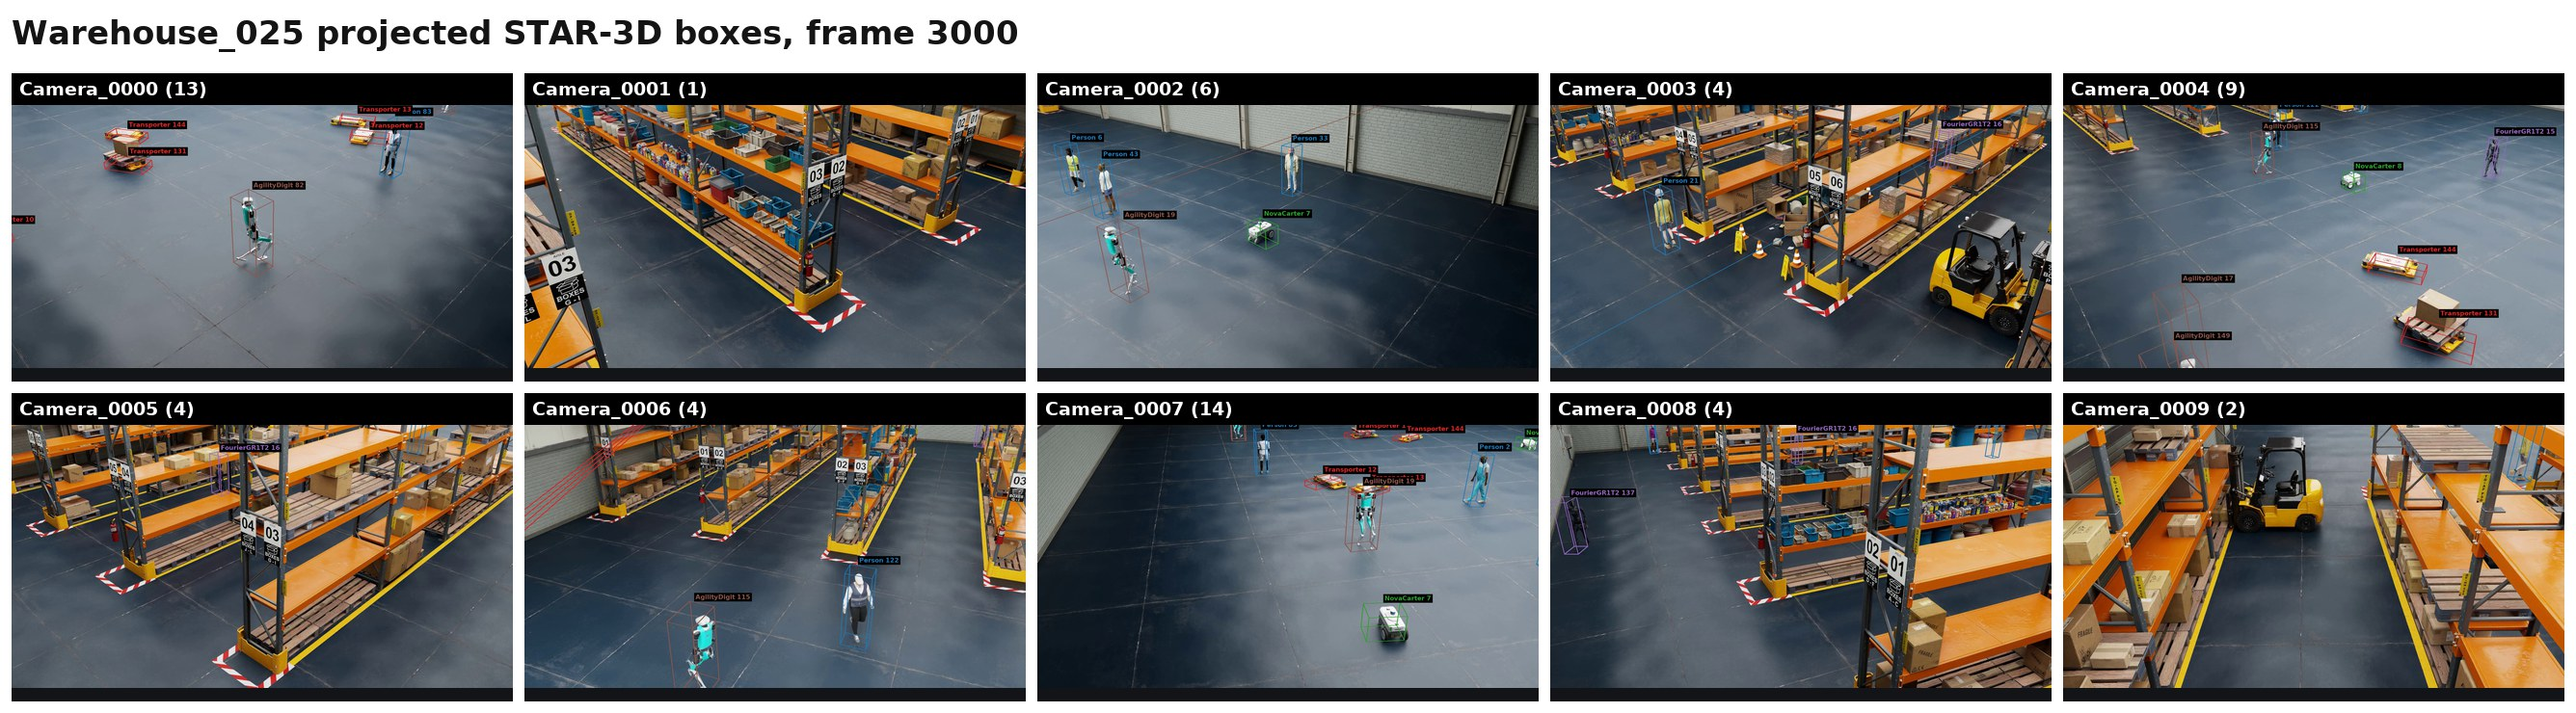
\includegraphics[width=\linewidth]{figures/qual_multicam_scene25_frame3000.jpg}
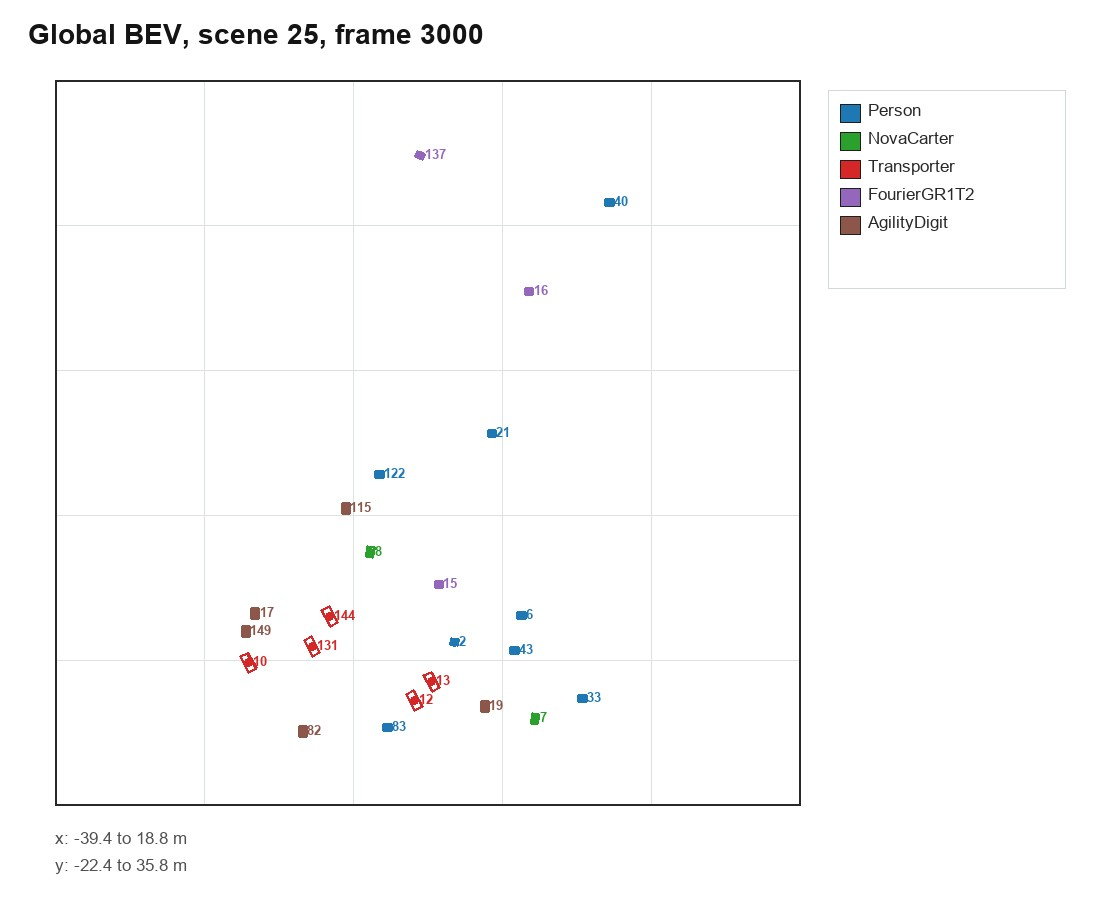
\includegraphics[width=0.48\linewidth]{figures/qual_bev_scene25_frame3000.jpg}
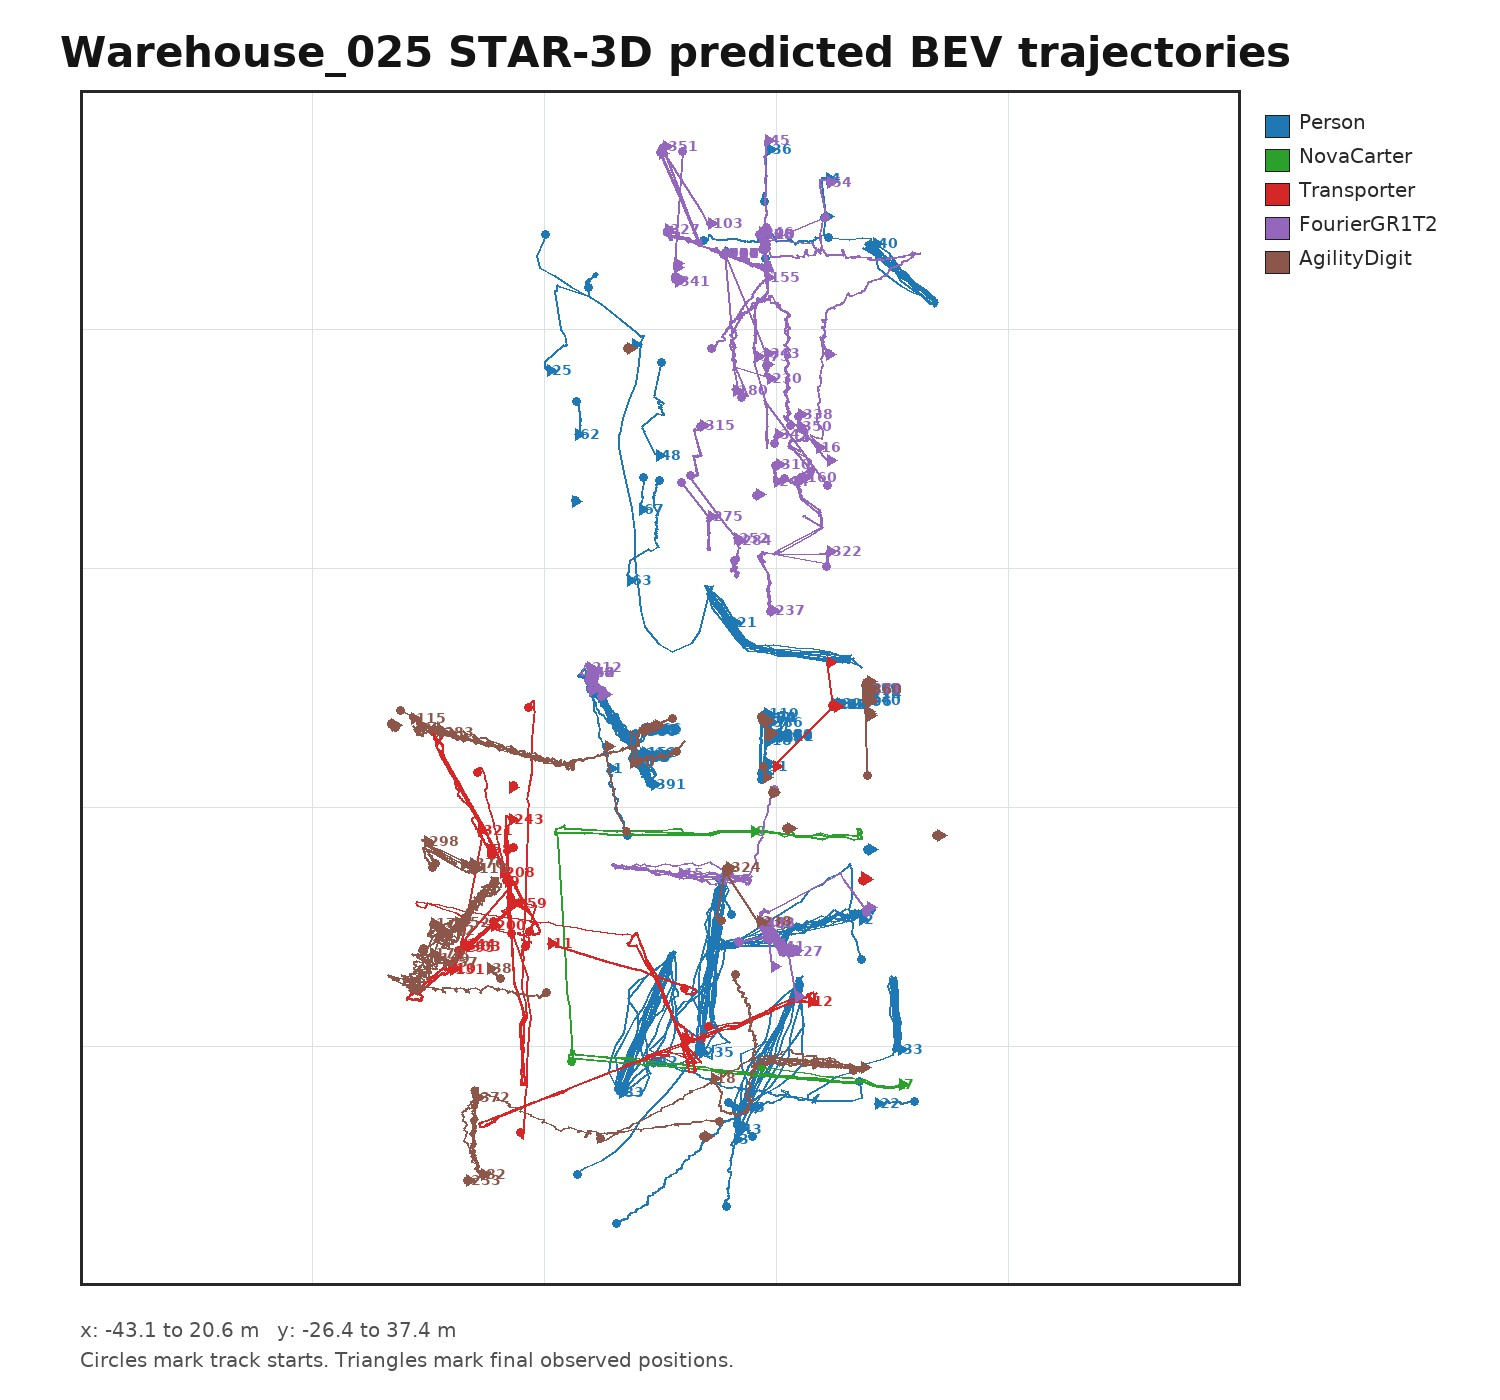
\includegraphics[width=0.48\linewidth]{figures/qual_bev_trajectories_scene25.jpg}
\caption{Qualitative STAR-3D predictions on a real Track 1 test scene. Top:
projected 3D boxes and shared global identities across synchronized camera
views. Bottom left: the same frame represented in the global BEV coordinate
system. Bottom right: long-horizon predicted trajectories for the scene. Colors
denote object classes.}
\label{fig:qualitative_bev}
\end{figure}

\subsection{Discussion}
\label{sec:exp_discussion}

The experiments show that RGB-based multi-camera 3D tracking is limited by the
interaction between detection, localization, and association. DetA and LocA can
increase without improving 3D HOTA when the new observations fragment identities.
Depth-based correction shows the same pattern: it can improve box placement, but it
must be calibrated with detector confidence and camera geometry to avoid harming
track continuity. STAR-3D therefore keeps the strongest high-resolution detector
evidence, uses calibration and class priors for stable lifting, and applies BEV
relinking only when the temporal and geometric support is strong.

\iffalse
The reason such papers will not be reviewed is that there is no provision for supervised revisions of manuscripts. 
The reviewing process cannot determine the suitability of the paper for presentation in 14 pages if it is reviewed in 16.


\subsection{Paper ID}
It is imperative that the paper ID is mentioned on each page of the manuscript of the review version.
Enter your paper ID in the appropriate place in the \LaTeX{} template (see \texttt{\%TODO REVIEW}).
The paper ID is a number automatically assigned to your submission when registering your paper submission on the submission site.


\subsection{Line Numbering}
\label{sec:line-numbering}
All lines should be numbered in the initial submission, as in this example document. 
This makes reviewing more efficient, because reviewers can refer to a line on a page. 
Line numbering is removed in the camera-ready version.


\section{Policies}
The policies governing the review process of ECCV \ECCVyear{} are detailed on the conference webpage (see \url{ https://eccv.ecva.net/Conferences/2026/SubmissionPolicies}), such as regarding confidentiality, dual submissions, double-blind reviewing, plagiarism, and more. 
By submitting a paper to ECCV, the authors acknowledge that they have read the submission policies and that the submission follows the rules set forth.

Accepted papers will be published in LNCS proceedings with Springer.
To that end, authors must follow the Springer Nature Code of Conduct for Authors (see \url{https://www.springernature.com/gp/authors/book-authors-code-of-conduct}).
We would like to draw particular attention to the policies regarding figures and illustrations, as well as ethical approval and informed consent, which are also reproduced on the ECCV website.


\section{Preserving Anonymity}
\label{sec:blind}
ECCV reviewing is double blind, in that authors do not know the names of the area chair/reviewers of their papers, and the area chairs/reviewers cannot, beyond reasonable doubt, infer the names of the authors from the submission and the additional material. 
You must not identify the authors nor provide links to websites that identify the authors, neither in the paper nor in the supplemental material.
If you need to cite a different paper of yours that is being submitted concurrently to ECCV, you should \emph{(1)} cite these papers anonymously, \emph{(2)} argue in the body of your paper why your ECCV paper is non-trivially different from these concurrent submissions, and \emph{(3)} include anonymized versions of those papers in the supplemental material.
Violation of any of these guidelines may lead to rejection without review. 

Many authors misunderstand the concept of anonymizing for blind review.
Blind review does not mean that one must remove citations to one's own work---in fact it is often impossible to review a paper unless the previous citations are known and available.

Blind review means that you do not use the words ``my'' or ``our'' when citing previous work.
That is all.
(But see below for tech reports.)

Saying ``this builds on the work of Lucy Smith [1]'' does not say that you are Lucy Smith;
it says that you are building on her work.
If you are Smith and Jones, do not say ``as we show in [7]'', say ``as Smith and Jones show in [7]'' and at the end of the paper, include reference 7 as you would any other cited work.

An example of a bad paper just asking to be rejected:
\begin{quote}
  \begin{center}
      An analysis of the frobnicatable foo filter.
  \end{center}

   In this paper we present a performance analysis of our previous paper [1], and show it to be inferior to all previously known methods.
   Why the previous paper was accepted without this analysis is beyond me.

   [1] Removed for blind review
\end{quote}

An example of an acceptable paper:
\begin{quote}
  \begin{center}
     An analysis of the frobnicatable foo filter.
  \end{center}

   In this paper we present a performance analysis of the  paper of Smith \etal [1], and show it to be inferior to all previously known methods.
   Why the previous paper was accepted without this analysis is beyond me.

   [1] Smith, L and Jones, C. ``The frobnicatable foo filter, a fundamental contribution to human knowledge''. Nature 381(12), 1-213.
\end{quote}

If you are making a submission to another conference at the same time, which covers similar or overlapping material, you may need to refer to that submission in order to explain the differences, just as you would if you had previously published related work.
In such cases, include the anonymized parallel submission [1] as supplemental material and cite it as
\begin{quote}
  [1] Authors. ``The frobnicatable foo filter'', ECCV \ECCVyear Submission ID 00324, Supplied as supplemental material {\tt 00324.pdf}.
\end{quote}

Finally, you may feel you need to tell the reader that more details can be found elsewhere, and refer them to a technical report.
For conference submissions, the paper must stand on its own, and not \emph{require} the reviewer to go to a tech report for further details.
Thus, you may say in the body of the paper ``further details may be found in~\cite{Anonymous24b}''.
Then submit the tech report as supplemental material.
Again, you may not assume the reviewers will read this material.

Sometimes your paper is about a problem, which you tested using a tool that is widely known to be restricted to a single institution.
For example, let's say it's 1969, you have solved a key problem on the Apollo lander, and you believe that the ECCV audience would like to hear about your
solution.
The work is a development of your celebrated 1968 paper entitled ``Zero-g frobnication: How being the only people in the world with access to the Apollo lander source code makes us a wow at parties'', by Zeus \etal.

You can handle this paper like any other.
Do not write ``We show how to improve our previous work [Anonymous, 1968].
This time we tested the algorithm on a lunar lander [name of lander removed for blind review]''.
That would be silly, and would immediately identify the authors.
Instead write the following:
\begin{quotation}
   We describe a system for zero-g frobnication.
   This system is new because it handles the following cases:
   A, B.  Previous systems [Zeus et al. 1968] did not  handle case B properly.
   Ours handles it by including a foo term in the bar integral.

   ...

   The proposed system was integrated with the Apollo lunar lander, and went all the way to the moon, don't you know.
   It displayed the following behaviours, which show how well we solved cases A and B: ...
\end{quotation}
As you can see, the above text follows standard scientific convention, reads better than the first version, and does not explicitly name you as the authors.
A reviewer might think it likely that the new paper was written by Zeus \etal, but cannot make any decision based on that guess.
He or she would have to be sure that no other authors could have been contracted to solve problem B.

For sake of anonymity, authors must omit acknowledgements in the review copy. 
They can be added later when you prepare the final copy.


\section{Formatting Guidelines}

\subsection{Headings}
Headings should be capitalized (\ie, nouns, verbs, and all other words except articles, prepositions, and conjunctions should be set with an initial capital) and should, with the exception of the title, be aligned to the left.
Only the first two levels of section headings should be numbered, as shown in \cref{tab:headings}.
The respective font sizes are also given in \cref{tab:headings}. 
Kindly refrain from using ``0'' when numbering your section headings.
Words joined by a hyphen are subject to a special rule. 
If the first word can stand alone, the second word should be capitalized.

\begin{table}[tb]
  \caption{Font sizes of headings. 
    Table captions should always be positioned \emph{above} the tables.
  }
  \label{tab:headings}
  \centering
  \begin{tabular}{@{}lll@{}}
    \toprule
    Heading level & Example & Font size and style\\
    \midrule
    Title (centered)  & {\Large\bf Lecture Notes \dots} & 14 point, bold\\
    1st-level heading & {\large\bf 1 Introduction} & 12 point, bold\\
    2nd-level heading & {\bf 2.1 Printing Area} & 10 point, bold\\
    3rd-level heading & {\bf Headings.} Text follows \dots & 10 point, bold\\
    4th-level heading & {\it Remark.} Text follows \dots & 10 point, italic\\
  \bottomrule
  \end{tabular}
\end{table}

Here are some examples of headings: 
``Criteria to Disprove Context-Freeness of Collage Languages'', ``On Correcting the Intrusion of Tracing Non-deterministic Programs by Software'', ``A User-Friendly and Extendable Data Distribution System'', ``Multi-flip Networks: Parallelizing GenSAT'', ``Self-determinations of Man''.


\subsection{Figures}
\label{sect:figures}
For \LaTeX{} users, we recommend integrating figures in your paper using the package \texttt{graphicx}.

It is essential that all illustrations are clear and legible. 
Vector graphics (rather than rasterized images) should be used for diagrams and schemas whenever possible. 
Please check that the lines in line drawings are not interrupted and have a constant width. 
Line drawings are to have a resolution of at least 800 dpi (preferably 1200 dpi).
Grids and details within figures must be clearly legible and may not be written one on top of the other. 
The lettering in figures should not use font sizes smaller than 6\:pt ($\sim$2\:mm character height). 

Figures should be numbered and should have a caption, which should always be positioned \emph{under} the figures, in contrast to the caption belonging to a table, which should always appear \emph{above} the table.
Figures and Tables should be cross-referred in the text.

If they are short, they are centered between the margins (\cf \cref{fig:short}). 
Longer captions, covering more than one line, are justified (\cref{fig:example} shows an example). 
Captions that do not constitute a full sentence, do not have a period.


\begin{figure}[tb]
  \centering
  \includegraphics[height=6.5cm]{eijkel2}
  \caption{One kernel at $x_s$ (\emph{dotted kernel}) or two kernels at $x_i$ and $x_j$ (\emph{left and right}) lead to the same summed estimate at $x_s$.
    This shows a figure consisting of different types of lines.
    Elements of the figure described in the caption should be set in italics, in parentheses, as shown in this sample caption. 
    The last sentence of a figure caption should generally end with a full stop, except when the caption is not a full sentence.
  }
  \label{fig:example}
\end{figure}

\begin{figure}[tb]
  \centering
  \begin{subfigure}{0.68\linewidth}
    \fbox{\rule{0pt}{0.5in} \rule{.9\linewidth}{0pt}}
    \caption{An example of a subfigure}
    \label{fig:short-a}
  \end{subfigure}
  \hfill
  \begin{subfigure}{0.28\linewidth}
    \fbox{\rule{0pt}{0.5in} \rule{.9\linewidth}{0pt}}
    \caption{Another example of a subfigure}
    \label{fig:short-b}
  \end{subfigure}
  \caption{Centered, short example caption}
  \label{fig:short}
\end{figure}

If possible (\eg, if you use \LaTeX) please define figures as floating objects. 
\LaTeX{} users, please avoid using the location parameter ``h'' for ``here''. 
If you have to insert a pagebreak before a figure, please ensure that the previous page is completely filled.


\subsection{Formulas}
Displayed equations or formulas are centered and set on a separate line (with an extra line or half line space above and below). 
Equations should be numbered for reference. 
The numbers should be consecutive within the contribution, with numbers enclosed in parentheses and set on the right margin.
For example,
\begin{align}
  \psi (u) & = \int_{0}^{T} \left[\frac{1}{2}
  \left(\Lambda_{0}^{-1} u,u\right) + N^{\ast} (-u)\right] \text{d}t \; \\
& = 0
\end{align}
and 
\begin{equation}
  E = m\cdot c^2.
  \label{eq:important}
\end{equation}
Please do not include section counters in the numbering.

Numbering equations makes reviewing more efficient, because reviewers can refer to a line on a page.  
It is important for readers to be able to refer to any particular equation.
Just because you did not refer to it in the text does not mean some future reader might not need to refer to it.
It is cumbersome to have to use circumlocutions like ``the equation second from the top of page 3''.
(Note that the ruler will not be present in the final copy, so is not an alternative to equation numbers).
All authors will benefit from reading Mermin's description of how to write mathematics:
\url{https://doi.org/10.1063/1.2811173}.

% No color equations in Springer publications.
Equations should never be in color and should be punctuated in the same way as ordinary text.
They should not be pasted in as figures.


\subsubsection{Lemmas, Propositions, and Theorems.}
The numbers accorded to lemmas, propositions, and theorems, \etc should appear in consecutive order, starting with Lemma 1. 
Please do not include section counters in the numbering like ``Theorem 1.1''.


\subsection{Footnotes.}
The superscript numeral used to refer to a footnote appears in the text either directly after the word to be discussed or -- in relation to a phrase or a sentence -- following the punctuation mark (comma, semicolon, or period).%
\footnote{The footnote numeral is set flush left and the text follows with the usual word spacing. 
  Second and subsequent lines are indented. 
}
For remarks pertaining to the title or the authors' names, in the header of a paper, symbols should be used instead of a number.
Please note that no footnotes may be included in the abstract.


\subsection{Cross References}
For the benefit of author(s) and readers, please use the
\begin{verbatim}
  \cref{...}
\end{verbatim}
command for cross-referencing to figures, tables, equations, or sections.
This will automatically insert the appropriate label alongside the cross reference as in this example:
\begin{quotation}
  To see how our method outperforms previous work, please see \cref{fig:example} and \cref{tab:headings}.
  It is also possible to refer to multiple targets as once, \eg~to \cref{fig:example,fig:short-a}.
  You may also return to \cref{sec:intro} or look at \cref{eq:important}.
\end{quotation}
If you do not wish to abbreviate the label, for example at the beginning of the sentence, you can use the
\begin{verbatim}
  \Cref{...}
\end{verbatim}
command. Here is an example:
\begin{quotation}
  \Cref{fig:example} is also quite important.
\end{quotation}


\subsection{Program Code}
Program listings or program commands in the text are normally set in typewriter font (\eg, \texttt{printf("Hello world!\textbackslash{}n");}).


\subsection{Citations}
Arabic numbers are used for citation, which is sequential either by order of citation or by alphabetical order of the references, depending on which sequence is used in the list of references. 
The reference numbers are given in brackets and are not superscript.
Please observe the following guidelines:
\begin{itemize}
\item Single citation: \cite{Anonymous24}
\item Multiple citation: \cite{Alpher02,Alpher03,Alpher05,Anonymous24b,Anonymous24}. 
  The numbers should be listed in numerical order.
  If you use the template as advised, this will be taken care of automatically.
\item If an author's name is used in the text: Alpher \cite{Alpher02} was the first \ldots
\end{itemize}
Please write all references using the Latin alphabet. If the title of the book you are referring to is, \eg, in Russian or Chinese, then please write (in Russian) or (in Chinese) at the end of the transcript or translation of the title.
All references cited in the text should be in the list of references and vice versa.

References should be formatted with the official LNCS reference style.
The \LaTeX{} template already takes care of that through the use of the \texttt{splncs04.bst} Bib\TeX{} style file.
Springer strongly encourages you to include DOIs (Digital Object Identifiers) in your references (\cf \cite{ECCV2022}). 
The DOI is a unique code allotted by the publisher to each online paper or journal article. 
It provides a stable way of finding published papers and their metadata. 
The insertion of DOIs increases the overall length of the references section, but this should not concern you as the reference section is not counted toward the page limit.


\subsection{Miscellaneous}
Compare the following:
\begin{center}
  \begin{tabular}{ll}
    \verb'$conf_a$'          & $\qquad conf_a$ \\
    \verb'$\mathit{conf}_a$' & $\qquad \mathit{conf}_a$
  \end{tabular}
\end{center}
See The \TeX book, p.\ 165.

The space after \eg, meaning ``for example'', should not be a sentence-ending space.
So \eg is correct, \emph{e.g.} is not.
The provided \verb'\eg' macro takes care of this.

When citing a multi-author paper, you may save space by using ``et alia'', 
shortened to ``\etal'' (not ``{\em et.\ al.}'' as ``{\em et\hskip 0.1em}'' is a complete word).
If you use the \verb'\etal' macro provided, then you need not worry about double periods when used at the end of a sentence as in Alpher \etal.
However, use it only when there are three or more authors.
Thus, the following is correct:
   ``Frobnication has been trendy lately.
   It was introduced by Alpher~\cite{Alpher02}, and subsequently developed by
   Alpher and Fotheringham-Smythe~\cite{Alpher03}, and Alpher \etal~\cite{Alpher04}.''

This is incorrect: ``... subsequently developed by Alpher \etal~\cite{Alpher03} ...'' because reference~\cite{Alpher03} has just two authors.


\subsection{Most Frequently Encountered Issues}
Please kindly use the checklist below to deal with some of the most frequently encountered issues in the latex files of ECCV submissions.

\begin{itemize}
\item I have removed all \verb| \vspace| and \verb|\hspace|  commands from my paper.
\item I have not used \verb|\cite| command in the abstract.
\item I have entered a correct \verb|\titlerunning{}| command and selected a meaningful short name for the paper.
\item I have used the same name spelling in all my papers accepted to ECCV and ECCV Workshops.
\item I have added acknowledgments without a section number, e.g. using the \verb|\section*{}| command.
\item Excluding references and acknowledgments, my paper is no longer than 14 pages.
\item I have not decreased the font size of any part of the paper (except tables) to fit into 14 pages, I understand Springer editors will remove such commands.
\end{itemize}


\section{Conclusion}
The paper ends with a conclusion. 

\clearpage\mbox{}Page \thepage\ of the manuscript.
\clearpage\mbox{}Page \thepage\ of the manuscript.
\clearpage\mbox{}Page \thepage\ of the manuscript.
\clearpage\mbox{}Page \thepage\ of the manuscript.
\clearpage\mbox{}Page \thepage\ of the manuscript. This is the last page.
\par\vfill\par
Now we have reached the maximum length of an ECCV \ECCVyear{} submission (excluding references and acknowledgements).
References should start immediately after the main text, but can continue past p.\ 14 if needed. 
\clearpage  % TODO FINAL: This \clearpage needs to be removed from both review and camera-ready versions.

\section*{Acknowledgements}
Please insert your acknowledgments here.

\fi

% ---- Bibliography ----
%
% BibTeX users should specify bibliography style 'splncs04'.
% References will then be sorted and formatted in the correct style.
%
\bibliographystyle{splncs04}
\bibliography{main}
\end{document}
